\documentclass{IEEEtran}
\usepackage[utf8]{inputenc}
\usepackage{tikz}
\usetikzlibrary{arrows.meta}
\usepackage{enumitem}
\usepackage{amsmath,amssymb,amsfonts}
\usepackage{mathtools}
\usepackage{bm}
\usepackage{graphicx}
\usepackage{cite}
\usepackage{hyperref}
\usepackage{float}
\usepackage{placeins}
\usepackage{tikz}
\usetikzlibrary{shapes.geometric, arrows.meta, positioning, fit, calc, backgrounds, shadows}

\title{A Unique Pipeline for Low Resolution Facial Recognition}
\author{Daniel Szurek, Brandon Nguyen}
\date{\today}

\begin{document}

\maketitle

\begin{abstract}
Low-resolution facial recognition (LRFR) remains a major challenge in real-world surveillance and security systems, since security cameras often capture subjects at extremely small spatial resolutions (e.g., 16×16 or 32×32). Modern facial recognition models are not designed to handle such low resolutions and perform much worse in these conditions. In this paper, we present a lightweight end-to-end pipeline that integrates identity-aware super-resolution with efficient facial recognition to address the very-low-resolution (VLR) face recognition problem. Our approach combines a Hybrid Transformer-CNN Deep Super-Resolution (DSR) network, utilizing Max-Feature-Map (MFM) activation for efficient feature selection and transformer attention for global context, with EdgeFace, a lightweight facial recognition backbone optimized for edge device deployment. To bridge the resolution domain gap, we incorporate multi-scale perceptual loss, identity cosine embedding loss, cross-photo identity consistency, and discriminative supervision, enabling the super-resolution model to reconstruct features that are explicitly relevant for identity identification. Evaluated on Labeled Faces in the Wild (LFW) and CMU Multi-PIE with probe images at 16×16, 24×24, and 32×32 resolutions, our pipeline demonstrates a consistent improvement in recognition accuracy over bicubic baselines. 
\end{abstract}

\begin{IEEEkeywords}
low-resolution face recognition, deep learning, super resolution
\end{IEEEkeywords}

\section{Introduction}

\renewcommand\thesubsection{\thesection.\Alph{subsection}}

Facial recognition has rapidly become a core component of modern security and surveillance infrastructures, offering capabilities ranging from access control to automated monitoring. However, many existing or low-cost systems cannot take full advantage of these advances due to limitations in their imaging hardware. Cameras mounted on buildings, street poles, or long-range checkpoints often capture faces at significant distances, producing extremely low-resolution images. Harsh lighting, motion blur, and inexpensive sensors further degrade visual quality, stripping away the discriminative detail needed for reliable identification. Together, these factors give rise to the very-low-resolution facial recognition (VLR-FR) challenge, where inputs may be as small as 16×16 or 32×32 pixels, which is far below the 112×112 resolution expected by current deep face recognition models.

Traditional face recognition pipelines, which are typically trained on high-resolution datasets like MS-Celeb-1M and VGGFace2, exhibit substantial performance degradation when presented with VLR inputs. This decline comes from two fundamental issues. First, severe downsampling removes essential discriminative features, including fine-grained textures, subtle expression patterns, and localized geometric structure, that modern recognition models rely on. Once these features are lost, they cannot be recovered. Second, the distribution shift between high-resolution training data and low-resolution test data creates a domain gap that deep networks struggle to correct. Simply upsampling VLR images with bicubic interpolation before recognition yields marginal improvements as it introduces smoothing artifacts without restoring the lost high-frequency details needed for accurate identification.

Super-resolution (SR) techniques offer a promising pathway to address VLR-FR by reconstructing high-resolution details from low-resolution inputs. However, conventional SR models optimized for perceptual quality metrics (PSNR, SSIM) do not necessarily preserve identity-discriminative features required for reliable recognition. A super-resolved face may appear visually convincing while still failing to produce embeddings that are consistent with those extracted from ground truth high-resolution images. This disconnect motivates the need for identity-aware super-resolution, SR models explicitly trained to recover and preserve the facial features that recognition networks depend upon for accurate matching.

A critical limitation in current super-resolution architectures lies in the trade-off between local texture recovery and global structural coherence. Purely Convolutional Neural Networks (CNNs) excel at extracting high-frequency local details but often struggle to capture long-range dependencies due to their limited receptive fields. In the context of VLR faces, this results in outputs that are sharp but geometrically distorted. For example, misaligned eyes or asymmetric jawlines. This confuses recognition models. Conversely, Vision Transformers (ViTs) utilize self-attention mechanisms to model global context effectively but can be computationally prohibitive for edge applications. This dichotomy necessitates a hybrid approach that leverages the efficiency of CNNs for feature extraction while utilizing lightweight transformer blocks to enforce global facial symmetry and structural integrity.

Furthermore, the deployment environment imposes strict constraints on model complexity. In real-world surveillance scenarios, transmitting high-bandwidth video streams to a centralized server for processing introduces significant latency and privacy vulnerabilities. To enable scalable and secure VLR-FR, the enhancement and recognition pipeline must be capable of running locally on edge devices (e.g., smart cameras or IoT gateways). This requirement precludes the use of massive generative models, such as diffusion probabilistic models or large GANs, which offer high visual fidelity but require computational resources unavailable on standard embedded hardware. Consequently, achieving a balance between low parameter count, real-time inference speed, and recognition accuracy becomes a paramount engineering challenge.

Our work is motivated by three key observations. First, the super-resolution and recognition stages should be jointly optimized rather than treated as independent modules, since decoupled training often results in mismatched feature distributions. Second, lightweight architectures are essential for deployment on edge devices with limited computing power, requiring models that balance efficiency with the ability to maintain recognition accuracy. Third, domain adaptation between SR outputs and the expectations of the recognition backbone has a substantial impact on end-to-end accuracy. To address these challenges, we propose a novel pipeline that couples a Hybrid Transformer–CNN Deep Super-Resolution (DSR) network with EdgeFace, a compact recognition backbone, unified through identity-preserving training objectives and cycle optimization.

\subsection{Novelty and Contributions}
We introduce a compact yet powerful pipeline designed specifically for very-low-resolution facial recognition. Our primary contribution is a Hybrid Transformer–CNN Deep Super-Resolution (DSR) architecture containing fewer than 5.5 million parameters. This model integrates the local feature extraction strengths of convolutional layers with the global context modeling ability of transformer attention, while employing Max-Feature-Map (MFM) activation to perform efficient channel-wise feature selection. Together, these components enable the network to hallucinate plausible facial structure while remaining lightweight enough for real-time deployment.

A second contribution lies in our identity-aware optimization strategy. Rather than relying solely on perceptual metrics such as PSNR or SSIM, we train the DSR network using a combination of multi-scale perceptual loss, identity cosine embedding loss, cross-photo identity consistency, and discriminative supervision. These objectives encourage the super-resolved images to retain features that align with the embedding space of the recognition model, improving identity preservation.

We further demonstrate that the proposed methodology generalizes across multiple levels of degradation by training separate DSR models for 16×16, 24×24, and 32×32 input resolutions. This scalability highlights the flexibility of our design for varying surveillance conditions and application requirements.

Finally, we conduct a comprehensive evaluation including Rank-1 accuracy, ROC-AUC, EER, and computational performance on both desktop hardware and edge devices. These results verify that our full pipeline operates in real time while outperforming bicubic upsampling baselines and offering meaningful improvements to recognition accuracy under severe resolution constraints.


\section{Related Work}

In this section, we review related works across three relevant areas, super-resolution methods, low-resolution face recognition techniques, and efficient recognition architectures for edge deployment, focusing on approaches that influenced the design of our pipeline and the key insights that shaped our methodological choices.

\subsection{Deep Learning for Super-Resolution}

Early deep learning approaches to single-image super-resolution (SISR) demonstrated that convolutional neural networks could learn an effective mapping from low to high-resolution images. A foundational example is SRCNN, introduced by Dong et al.~\cite{srcnn}, which established CNN-based SR as a viable framework. 

The work most relevant to our work, however, is ESRGAN~\cite{esrgan}, which introduced perceptual-driven adversarial training and demonstrated that global context is necessary for reconstructing fine image details. ESRGAN’s emphasis on perceptual similarity motivated our adoption of multi-scale perceptual loss and informed our decision to incorporate transformer attention into our DSR architecture. Although effective for improving visual quality, these SR approaches do not explicitly preserve identity features, limiting their usefulness for VLR face recognition.

\subsection{Low-Resolution Face Recognition}

Among low-resolution face recognition approaches, the most influential for our work is the Deep Super-Resolution (DSR) architecture proposed by He et al.~\cite{dsr}. Their use of residual dense blocks and identity supervision demonstrated that SR models optimized for recognition outperform those targeting appearance-quality metrics. 
Another relevant contribution is Coupled-GAN by Li et al.~\cite{coupledgan}, which jointly trained SR and recognition networks via a shared latent space. While complex, Coupled-GAN reinforced the importance of aligning SR outputs with the recognition model's embedding space. These insights guided our design of identity-aware losses and validated our choice to tightly couple SR with recognition.

\subsection{Efficient Face Recognition Models}

Given our goal of achieving real-time inference on edge devices, our work focuses exclusively on EdgeFace~\cite{edgeface}, a lightweight facial recognition model built on a hybrid Transformer–CNN architecture. The EdgeFace-XXS variant, which we employ, contains only 1.24M parameters and produces 512-dimensional embeddings, offering strong performance while remaining computationally efficient. Studying EdgeFace provided two key insights. First, that global context modeling can be achieved without large parameter counts, informing our transformer-based DSR design. Second, recognition backbones optimized for low-power devices are essential for practical deployment.


\section{Methodology}

Our pipeline consists of three key components: a Hybrid Transformer-CNN DSR network for upsampling VLR inputs, the EdgeFace facial recognition backbone, and a cycle training strategy that jointly optimizes both stages.

\subsection{Hybrid Transformer-CNN DSR Network}

\subsubsection{Architecture}

The DSR network employs a Hybrid Transformer-CNN architecture designed to capture both local details and global context while maintaining efficiency. Our implementation uses resolution-specific configurations to balance performance and parameter count (\textless 5.5M). As seen in Figure~\ref{fig:arch}, we first employ a 3×3 convolutional layer to map RGB input to a base channel space (96 for 16×16, 112 for 24×24, 120 for 32×32) for shallow feature extraction. For deep feature extraction, our model contains a sequence of Residual Blocks (8 for 16×16, 6 for 24×24, 5 for 32×32) employing Max-Feature-Map (MFM) activation. MFM acts as a feature selection mechanism, splitting channels and taking the maximum to suppress noise and enhance discriminative features. To minimize parameter count while maintaining super-resolution performance, our implementation features Transformer Attention Blocks (4 for 16×16/24×24, 3 for 32×32) with multi-head self-attention (8 heads) and MLP expansion ratio of 2.0. This captures long-range dependencies crucial for hallucinating plausible facial structures. After feature extraction and global context, pixel shuffle layers~\cite{pixelshuffle} progressively upscale features to the target resolution. Finally, a 3x3 convolution produces the RGB output to perform facial recognition.

\begin{figure*}[ht!]
\centering
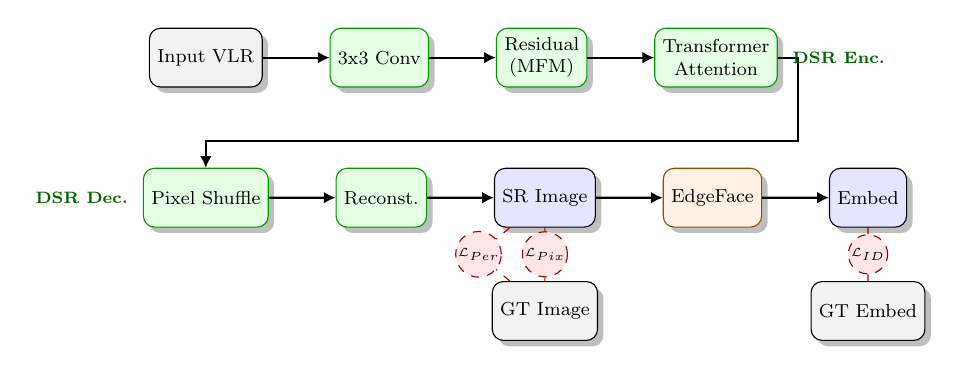
\begin{tikzpicture}[
    scale=0.85, transform shape,
    node distance=1.0cm and 1.0cm,
    >={Latex[width=1.5mm,length=1.5mm]},
    block/.style={rectangle, draw, fill=white, text centered, rounded corners, minimum height=2.5em, drop shadow, font=\footnotesize},
    dsr/.style={block, fill=green!10, draw=green!60!black},
    recog/.style={block, fill=orange!10, draw=orange!60!black},
    loss/.style={circle, draw=red!60!black, fill=red!10, inner sep=0.5pt, font=\tiny, dashed},
    line/.style={draw, ->, thick}
]
    \node (input) [block, fill=gray!10] {Input VLR};
    \node (conv1) [dsr, right=of input] {3x3 Conv};
    \node (res) [dsr, right=of conv1, align=center] {Residual\\(MFM)};
    \node (trans) [dsr, right=of res, align=center] {Transformer\\Attention};


    \node (pixel) [dsr, below=1.2cm of input] {Pixel Shuffle};
    \node (conv2) [dsr, right=of pixel] {Reconst.};
    \node (srout) [block, right=of conv2, fill=blue!10] {SR Image};
    \node (edgeface) [recog, right=of srout] {EdgeFace};
    \node (embed) [block, right=of edgeface, fill=blue!10] {Embed};


    \node (hr) [block, below=0.8cm of srout, fill=gray!10] {GT Image};
    \node (hrembed) [block, below=0.8cm of embed, fill=gray!10] {GT Embed};

    \draw[line] (input) -- (conv1);
    \draw[line] (conv1) -- (res);
    \draw[line] (res) -- (trans);

    \draw[line] (trans.east) -- ++(0.3,0) |- ($(pixel.north)+(0,0.4)$) -| (pixel.north);

    \draw[line] (pixel) -- (conv2);
    \draw[line] (conv2) -- (srout);
    \draw[line] (srout) -- (edgeface);
    \draw[line] (edgeface) -- (embed);

    \path (srout) -- (hr) coordinate[midway] (mid_img);
    \node (l1) [loss] at (mid_img) {$\mathcal{L}_{Pix}$};
    \node (lp) [loss, left=0.3cm of l1] {$\mathcal{L}_{Per}$};
    
    \draw[dashed, red!60!black] (srout) -- (l1);
    \draw[dashed, red!60!black] (hr) -- (l1);
    \draw[dashed, red!60!black] (srout) -- (lp);
    \draw[dashed, red!60!black] (hr) -- (lp);

    \path (embed) -- (hrembed) coordinate[midway] (mid_id);
    \node (lid) [loss] at (mid_id) {$\mathcal{L}_{ID}$};
    
    \draw[dashed, red!60!black] (embed) -- (lid);
    \draw[dashed, red!60!black] (hrembed) -- (lid);

    \node[right=0.1cm of trans, font=\bfseries\scriptsize, text=green!40!black] {DSR Enc.};
    \node[left=0.1cm of pixel, font=\bfseries\scriptsize, text=green!40!black] {DSR Dec.};

\end{tikzpicture}
\caption{The proposed end-to-end pipeline. The VLR input is processed by the DSR network featuring MFM activation and Transformer attention. The super-resolved output is passed to EdgeFace for embedding verification. Training is supervised by pixel, perceptual, and identity losses.}
\label{fig:arch}
\end{figure*}


\subsubsection{Training Objectives}

DSR training employs a comprehensive loss function ($\mathcal{L}_{\text{DSR}}$) weighting identity preservation over pure pixel fidelity:

\begin{equation}
\mathcal{L}_{\text{DSR}} = \lambda_{\text{L1}}\mathcal{L}_{\text{L1}} + \lambda_{\text{P}}\mathcal{L}_{\text{P}} + \lambda_{\text{ID}}\mathcal{L}_{\text{ID}} + \lambda_{\text{Disc}}\mathcal{L}_{\text{Disc}} + \lambda_{\text{TV}}\mathcal{L}_{\text{TV}}
\end{equation}

\subsubsection{Loss Function Formalization}
To ensure the DSR network hallucinates identity-consistent details, we define the constituent components of our objective function $\mathcal{L}_{\text{DSR}}$ as follows.

\paragraph{Pixel-wise Loss ($\mathcal{L}_{\text{L1}}$)}
We utilize the $L_1$ norm rather than $L_2$ (MSE) to prevent over-smoothing of high-frequency details. Given the super-resolved output $I_{SR}$ and the ground truth high-resolution image $I_{HR}$:
\begin{equation}
    \mathcal{L}_{\text{L1}} = \frac{1}{HW} \sum_{i=1}^{H} \sum_{j=1}^{W} |I_{HR}^{(i,j)} - I_{SR}^{(i,j)}|
\end{equation}

\paragraph{Perceptual Loss ($\mathcal{L}_{\text{P}}$)}
Pixel-wise metrics do not capture semantic similarity. We extract features using a pre-trained VGG-19 network $\phi$. We minimize the Euclidean distance between feature maps at layer $j$ (specifically \texttt{relu5\_4}):
\begin{equation}
    \mathcal{L}_{\text{P}} = \frac{1}{C_j H_j W_j} || \phi_j(I_{HR}) - \phi_j(I_{SR}) ||^2_2
\end{equation}

\paragraph{Identity Preserving Loss ($\mathcal{L}_{\text{ID}}$)}
This is the most critical component for the recognition pipeline. We employ a pre-trained face recognition encoder $\psi$ (EdgeFace-XXS) to extract 512-dimensional embeddings $z_{HR} = \psi(I_{HR})$ and $z_{SR} = \psi(I_{SR})$. We utilize a cosine similarity metric to maximize the alignment of these embeddings in the hypersphere:
\begin{equation}
    \mathcal{L}_{\text{ID}} = 1 - \cos(z_{HR}, z_{SR}) = 1 - \frac{z_{HR} \cdot z_{SR}}{||z_{HR}||_2 \cdot ||z_{SR}||_2}
\end{equation}
By minimizing this angular distance, we force the DSR network to prioritize facial features that dictate identity (e.g., eye shape, bone structure) over irrelevant background textures.

First, we calculate the loss of visual fidelity via pixel loss and perceptual loss. These are defined as the L1 distance between SR and HR images and Multi-scale VGG-19 feature distance, respectively. In the loss function above, they are incorporated as $\lambda_{\text{L1}}=1.0$ for pixel loss, and $\lambda_{\text{P}}=0.02$ signifying perceptual loss.
Then, we calculate the loss from EdgeFace's ability to verify the subject. This is weighted the most in our loss function. We employ an identity loss $\mathcal{L}_{\text{ID}}$, which is composed of Cosine Similarity ($\lambda=15.0-18.0$), Cross-Photo Consistency ($\lambda=3.0-4.0$), Embedding Magnitude ($\lambda=0.15$), and Feature Correlation ($\lambda=2.0-3.0$) losses. This ensures that EdgeFace classifies the subject in the upscaled image as the same subject in the ground truth high resolution image. Next, to ensure that our model does not make each subject in its super-resolved images similar to each other, we incorporate a discriminative loss $\lambda_{\text{Disc}}=8.0$, which ensures SR outputs of different identities remain separable in embedding space. Finally, we include a total variation loss $\lambda_{\text{TV}}=10^{-5}$, which is simply defined as regularization for spatial smoothness.

\subsubsection{Training Configuration}

DSR is trained for 150 epochs (with a stop patience of 20 epochs) using the AdamW optimizer with a OneCycleLR scheduler (max LR $4 \times 10^{-4}$). We employ mixed-precision training (BF16/FP16) and gradient clipping (norm 1.0). Data augmentation includes MixUp, CutMix, horizontal flipping, rotation, and color jitter to improve robustness. During our training, we found that all models tended to converge after approximately 70 epochs. 

\subsubsection{Implementation}
Our final implementation attempted to mirror a real-world scenario as closely as possible with the resources allowed. We created a software application that captured photographs through a Logitech C920s webcam, scaled those photographs to the proper input resolutions, and processed them through our pipeline. The application allowed for gallery subject registration and matched input photographs to subjects registered in the gallery. This application was tested on a Raspberry Pi 5 and a home desktop computer to mimic hardware available in real-world scenarios. The performance of our pipeline in this application will be detailed in Section IV. Experiments and Results.

\begin{figure}[h!]
    \centering
    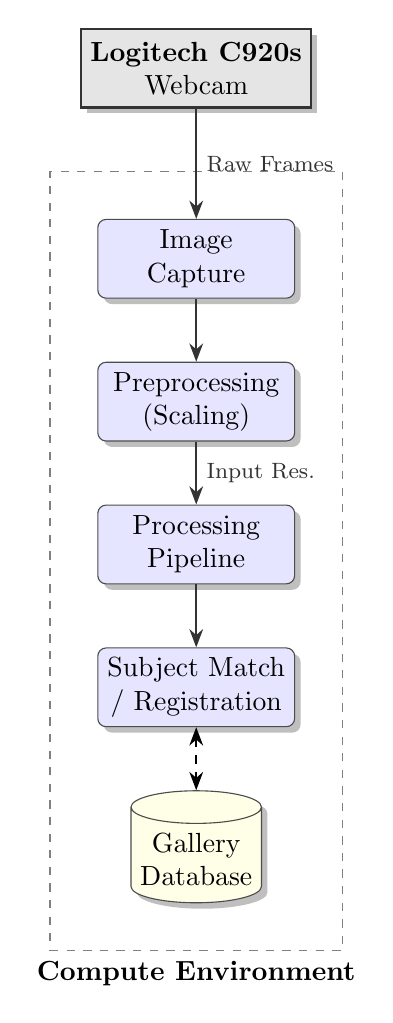
\begin{tikzpicture}[
        node distance=0.8cm, 
        >=Stealth,
        process/.style={
            rectangle, 
            minimum width=2.5cm, 
            minimum height=1cm, 
            align=center, 
            draw=black!70, 
            fill=blue!10, 
            rounded corners=3pt,
            drop shadow
        },
        hardware/.style={
            rectangle, 
            minimum width=2.5cm, 
            minimum height=1cm, 
            align=center, 
            draw=black!80, 
            fill=gray!20, 
            thick,
            drop shadow
        },
        database/.style={
            cylinder, 
            shape border rotate=90, 
            draw=black!70, 
            aspect=0.25, 
            fill=yellow!10, 
            minimum height=1.2cm, 
            minimum width=1.5cm, 
            align=center, 
            drop shadow
        },
        arrow/.style={
            ->, 
            thick, 
            color=black!80
        }
    ]

    
    \node (camera) [hardware] {\textbf{Logitech C920s} \\ Webcam};

    \node (capture) [process, below=1.4cm of camera] {Image \\ Capture};

    \node (scaling) [process, below=of capture] {Preprocessing \\ (Scaling)};

    \node (pipeline) [process, below=of scaling] {Processing \\ Pipeline};

    \node (matcher) [process, below=of pipeline] {Subject Match \\ / Registration};
    
    \node (gallery) [database, below=of matcher] {Gallery \\ Database};

    
    \begin{scope}[on background layer]
        \node (compute_env) [
            draw=black!50, 
            dashed, 
            inner sep=0.6cm, 
            fill=white, 
            fit=(capture) (scaling) (pipeline) (matcher) (gallery),
            label={[anchor=north]south:\textbf{Compute Environment}} 
        ] {};
    \end{scope}

    \draw [arrow] (camera) -- node[midway, right, font=\footnotesize] {Raw Frames} (capture);

    \draw [arrow] (capture) -- (scaling);

    \draw [arrow] (scaling) -- node[midway, right, font=\footnotesize] {Input Res.} (pipeline);

    \draw [arrow] (pipeline) -- (matcher);

    \draw [<->, thick, dashed] (matcher) -- (gallery);

    \end{tikzpicture}
    \caption{Implementation application architecture.}
    \label{fig:implementation_flow}
\end{figure}

\subsection{EdgeFace Recognition Network}

\subsubsection{Architecture}

EdgeFace employs a lightweight bottleneck design optimized for mobile deployment. It uses Lightweight Depthwise Convolution (LDC) blocks to reduce FLOPs while preserving expressive power. We use the EdgeFace-XXS variant which produces 512-dimensional embeddings.

\subsubsection{ArcFace Metric Learning}

For fine-tuning EdgeFace on DSR outputs, we employ ArcFace~\cite{arcface} additive angular margin loss ($s=64, m=0.5$) to encourage intra-class compactness and inter-class separability.

\subsection{Cycle Training Strategy}

Early on in our research process, our pipeline employed a three-phase cycle training strategy to co-adapt the super-resolution and recognition models. In the first phase, we train the hybrid DSR using the default pretrained EdgeFace-XXS as the identity supervisor. This establishes a baseline SR capability that respects the original embedding space. In the second phase, we fine-tune EdgeFace on the DSR outputs from Phase 1. This adapts the recognition model to the specific distribution of super-resolved images, improving its robustness to artifacts and missing details. Finally, we retrain the Hybrid DSR using the fine-tuned EdgeFace from Phase 2 as the supervisor. The DSR network now learns to produce features that are most discriminative for the adapted recognition model.

This cycle was intended to make EdgeFace more robust for our specific use case. Unfortunately, we found that this cyclic training methodology consistently reduced our overall performance by a factor of nearly 20 percent in some cases. We did not have enough time to investigate this phenomenon fully, but we believe this behavior may be attributed to overfitting our dataset and a suboptimal learning rate. Future work could include tuning the learning rate and using a more robust dataset to improve performance. 

\section{Experiments and Results}

In this section, we will discuss our dataset, experimentation methodology, and the results yielded from our test suite. We achieved competitive recognition results on a large subject number test gallery while maintaining a small parameter count of less than 5.5M for all three models. However, even with these results, we still recognize some limitations of this model. Therefore, we will also delve into these factors at the end of the section.

\subsection{Datasets}

We evaluate our pipeline on Labeled Faces in the Wild (LFW)~\cite{lfw}  and CMU Multi-PIE~\cite{multipie}, splitting the images into three categories: training, validation, and testing. In our testing subset, there were 16,708 images of 1,736 independent subjects. For each subject, we select all original images as high-resolution (HR) references, resized to 112×112 for EdgeFace recognition input.

These datasets were chosen for their large amount of subject photographs and their labeled nature. CMU Multi-PIE contains thousands of labeled images of subjects from various angles, while LFW contains images of subjects in various positions and angles, which would reflect a surveillance camera image more accurately.

Very-low-resolution (VLR) probes are synthesized by downsampling HR images using bicubic interpolation to 16×16, 24×24, and 32×32 pixels.

The authors recognize that the downsampling methodology is an idealized scenario. Real-world surveillance footage may contain different artifacts introduced via the camera's small sensor size or distance between the subject and itself. For the purposes of this study, we employed a proof-of-concept approach. 

\subsection{Evaluation Metrics}

Recognition performance is measured using Rank-1 Accuracy, ROC-AUC, EER, and True Accept Rate (TAR) at fixed False Accept Rate (FAR). We report accuracy at threshold $\tau = 0.35$.

\subsection{Results and Analysis}

\subsubsection{Quantitative Performance}

Table~\ref{tab:main_results} summarizes recognition and reconstruction performance across three VLR input resolutions:

\begin{table}[h]
\centering
\caption{Recognition and Super-Resolution Performance}
\label{tab:main_results}
\setlength{\tabcolsep}{3pt} 
\begin{tabular}{lcccccc}
\hline
\textbf{Resolution} & \textbf{Method} & \textbf{R1 Acc.} & \textbf{ROC-AUC} & \textbf{EER} & \textbf{PSNR/SSIM} & \textbf{1:1 Acc.} \\
\hline
16×16 & DSR & 38.0\% & 0.975 & 6.91\% & 30.8/0.807 & 99.43\%\\
 & Bicubic & 32.0\% & 0.971 & 7.46\% & 32.3/0.758 & 99.43\%\\
24×24 & DSR & 44.2\% & 0.984 & 5.12\% & 32.1/0.883 & 99.46\%\\
 & Bicubic & 41.7\% & 0.976 & 6.72\% & 33.7/0.852 & 99.45\% \\
32×32 & DSR & 47.5\% & 0.986 & 4.47\% & 32.9/0.923 & 99.56\%\\
 & Bicubic & 45.9\% & 0.983 & 5.24\% & 35.0/0.908 & 99.55\% \\
\hline
\end{tabular}
\end{table}
\begin{figure}
    \centering
    \includegraphics[width=1.0\linewidth]{Screenshot 2025-12-08 164951.png}
    \caption{ROC Curves}
    \label{fig:ROC}
\end{figure}

\begin{figure*}
    \centering
    \includegraphics[width=0.7\linewidth]{Screenshot 2025-12-08 165052.png}
    \caption{Example Output}
    \label{fig:ModelOutput}
\end{figure*}

Our pipeline achieves its best performance at 32×32 VLR input. Smaller input resolutions show degraded recognition, indicating the challenge of information loss at extreme downsampling. Super-resolution quality (PSNR/SSIM) generally improves with larger inputs.

\subsubsection{Qualitative Analysis}

Visual inspection of super-resolved outputs suggests that identity-aware training produces sharper facial features compared to generic methods. Our results indicate that PSNR/SSIM do not correlate perfectly with recognition performance - while 32×32 achieves high PSNR and SSIM, the corresponding Rank-1 accuracy remains modest, indicating fundamental challenges in very-low-resolution face recognition beyond reconstruction quality. This is an expected, if not desired, feature of our upscaling model. The training methodology focused more on the recognition performance of the model rather than purely qualitative super resolution. Because of this focus on a singular use case, we believe our model is superior for recognition tasks. Output of our super-resolution model can be found in Figure~\ref{fig:ModelOutput}.

\subsubsection{Computational Efficiency}

\begin{table}[h]
\centering
\caption{Super-Resolution Performance}
\label{tab:performance}
\begin{tabular}{lcccc}
\hline
\textbf{VLR Size} & \textbf{Total Time} & \textbf{Upscaling} & \textbf{Recognition} & \textbf{FPS} \\
\hline
16×16 & 18.4 ms & 7.7 ms & 10.8 ms & 54 \\
24×24 & 20.8 ms & 7.2 ms & 13.6 ms & 48 \\
32×32 & 19.0 ms & 5.4 ms & 13.7 ms & 53 \\
\hline
\end{tabular}
\end{table}

We tested our model on a desktop computer outfitted with an NVIDIA GeForce RTX 3060 Ti, 32 gigabytes of RAM, and an AMD Ryzen 7 5800X 8-Core Processor. As seen in \ref{tab:performance}, our full pipeline executed in real time at an average of 51.67 frames per second (FPS) across all three models. The bottleneck of pipeline performance was the recognition model. Further testing on a Raspberry Pi 5 with 4 gigabytes of RAM was a more accurate representation of edge case performance. On this hardware, we were still able to achieve real-time performance, with our pipeline outputting a verification score at approximately 1 fps.

\subsubsection{Comparison to Existing Methods}

We tested our model against a bicubic upscaling method. As seen in \ref{tab:main_results}, our model consistently outperformed the basic method. While 1:1 accuracy is relatively consistent across all methods tested (showing the power of EdgeFace's recognition more so than that of our super-resolution method), our models' strengths are seen when viewing results of large-scale gallery identification (Rank-1 Accuracy, Receiver Operating Characteristic Area Under Curve, Equal Error Rate). Here, we can see that our model achieves a score of up to six percentage points higher than that of the simple method in Rank-1 Accuracy, and ROC-AUC and EER metrics are also improved upon. These results were calculated by allowing EdgeFace to predict the identity of a subject in a gallery of 16,708 images of 1,736 subjects. The number of images per subject varied, with CMU Multi-Pie having some subjects with over 
500 images, while LFW had certain subjects with only one. With this test dataset being as diverse as it is, it is impressive that the pipeline correctly identified over 800 subjects. Furthermore, comparing against more advanced methods such as LightCNN-v29, whose listed 1:1 accuracy is 98.98\% and Rank-1 accuracy is listed as 41.36\%, we see how our proposed pipeline outperforms modern models while maintaining a lightweight architecture. 


\subsubsection{Failure Case Analysis}

While our model achieved competitive metrics in our idealized test scenario, per-subject accuracy variance still exists and is observed across the test set. A common failure mode includes VLR probes where extreme downsampling destroys facial structure, which unfortunately cannot be avoided in this low resolution problem domain. Similarly, subjects with similar facial geometry leading to inter-subject confusion is a common error within our implementation. Occasionally, our DSR model introduced smoothing artifacts that obscure discriminative features. This could be fixed with further tuning and training. Finally, a large factor in our results was a very large test set. The low Rank-1 accuracy indicates that even with super-resolution, identification from such degraded inputs remains extremely challenging, especially with a test set of over 1,500 subjects. However, for 1:1 verification, our models consistently achieved 99\% accuracy, exhibiting good performance in small gallery identification scenarios.

\section{Ethical Considerations}
The development of super-resolution and facial recognition technologies carries inherent ethical risks regarding privacy and potential misuse. While our pipeline is designed to enhance security in legitimate surveillance scenarios, such as identifying authorized personnel in low-bandwidth environments, it is crucial to address the risk of ``hallucination.''

Deep generative models, including our DSR network, can occasionally generate facial features that do not exist in the source image, potentially leading to false positives in identification. To mitigate this, our use of Identity Loss ($\mathcal{L}_{\text{ID}}$) specifically constrains the model to stay within the identity manifold of the subject, reducing the likelihood of generating a generic or incorrect face. Furthermore, we emphasize that VLR-FR systems should be used as a ``human-in-the-loop'' support tool rather than a fully autonomous decision-maker, particularly in high-stakes environments. We also acknowledge the bias inherent in public datasets like LFW and Multi-PIE; future deployment would require training on diverse datasets to ensure equitable performance across all demographics.

\section{Conclusion and Future Work}

This paper presented a pipeline for very-low-resolution facial recognition combining identity-aware super-resolution with lightweight recognition networks. Our key contributions include: (1) a small, efficient, and effective resolution-adaptive Hybrid DSR architectures trained with multi-scale perceptual and identity-preserving losses, (2) integration with EdgeFace-XXS for efficient embedding extraction, and (3) comprehensive evaluation across three VLR resolutions. Our implementation ranks amongst the smallest and most efficient super resolution models while still maintaining competitive accuracy scores.

\textbf{Limitations:} While 1:1 verification is near-perfect, Rank-1 identification accuracy for large-scale subject galleries remains below desirable thresholds. This accuracy must be improved before real-world deployment if subject galleries larger than 1,000 are desired. This model is also biased towards subjects photographed in the same manner as the CMU Multi-PIE dataset, which does not reflect real-world surveillance camera footage. 

Therefore, we suggest as future work to train with a dataset with more uniform subject counts. In the same vein, one could fine tune the model on surveillance-style datasets to ensure that the model performs as expected in its desired use case. A custom facial recognition model trained on DSR output to replace EdgeFace within this pipeline could also prove beneficial to final metrics. Finally, although our attempts were not successful, we believe that cyclical training still holds potential. With further experimentation, fine-tuning the DSR model on the custom recognition network may lead to improved performance.


\section*{Acknowledgments}

We thank the CMU Multi-PIE and LFW teams for providing the facial image datasets, and the EdgeFace authors for releasing trained model weights.

\bibliographystyle{IEEEtran}
\bibliography{references}

\end{document}